\documentclass[sigconf]{acmart}

\usepackage{booktabs} % For formal tables

\usepackage{amsmath}
\usepackage{float}
\usepackage{hyperref}
\usepackage{listings}
\usepackage{algorithm}
\usepackage[noend]{algpseudocode}
\usepackage{graphicx}
\usepackage{courier}
\usepackage{float}
\usepackage{color}
\usepackage[margin=10pt,font=small,labelfont=bf,
  labelsep=endash]{caption}
\usepackage{ulem}

\usepackage{syntax} % for writing BNF grammar

\usepackage{forest}
\usepackage{framed}

\usepackage{tikz}
\usetikzlibrary{matrix}
\usetikzlibrary{shapes.multipart}
\usetikzlibrary{patterns}
\usetikzlibrary{positioning,fit,calc}
\usetikzlibrary{decorations.pathmorphing}
\usetikzlibrary{decorations.pathreplacing}
\usetikzlibrary{quotes}
\usetikzlibrary{graphs}
\usetikzlibrary{arrows.meta}
\usetikzlibrary{shapes}
% \usetikzlibrary{graphs,graphdrawing}
% \usegdlibrary{layered}
% \usetikzlibrary{graphdrawing,graphs,calc}
% \usegdlibrary{layered}

\usepackage{smartdiagram}

% \usetikzlibrary{external}
% \tikzexternalize % activate!
% \tikzset{external/force remake}

%% To generate figure, uncomment above three lines, and execute:
%% pdflatex -shell-escape helium.tex

\usepackage{csvsimple}
\usepackage{multirow}


\lstset{basicstyle=\footnotesize\ttfamily,breaklines=true}
% \lstset{frame=b}
\lstset{float,floatplacement=H,captionpos=b}
% \lstset{numbers=left}
\lstset{language=C}
\lstset{showstringspaces=false}
\lstset{breakindent=10pt}
% \lstset{framextopmargin=10pt}
% \lstset{framextopmargin=50pt,frame=t}
% \lstset{float=htb,language=C,frame=single, basicstyle=\small, stringstyle=\ttfamily}
% \lstset{escapeinside={(*@}{@*)}}
% \usepackage{xcolor}
\lstdefinestyle{base}{
  language=C,
  emptylines=1,
  breaklines=true,
  aboveskip=0em,
  belowskip=0em,
  % float,
  % floatplacement=H,
  basicstyle=\footnotesize\ttfamily\color{black},
  moredelim=**[is][\color{blue}]{@}{@},
  moredelim=**[is][\color{purple}]{~1}{~1},
  moredelim=**[is][\color{brown}]{~2}{~2},
  moredelim=**[is][\color{gray}]{~3}{~3},
  moredelim=**[is][\color{orange}]{~4}{~4},
  moredelim=**[is][\color{violet}]{~5}{~5},
}
\lstdefinestyle{graycode} {
  language=C,
  emptylines=1,
  breaklines=true,
  basicstyle=\footnotesize\ttfamily\color{gray!50},
  moredelim=**[is][\color{blue}]{@}{@},
}
\lstset{style=base}


\usepackage{enumitem}

\begin{document}
\title{Test}


\begin{figure*}
  \centering
  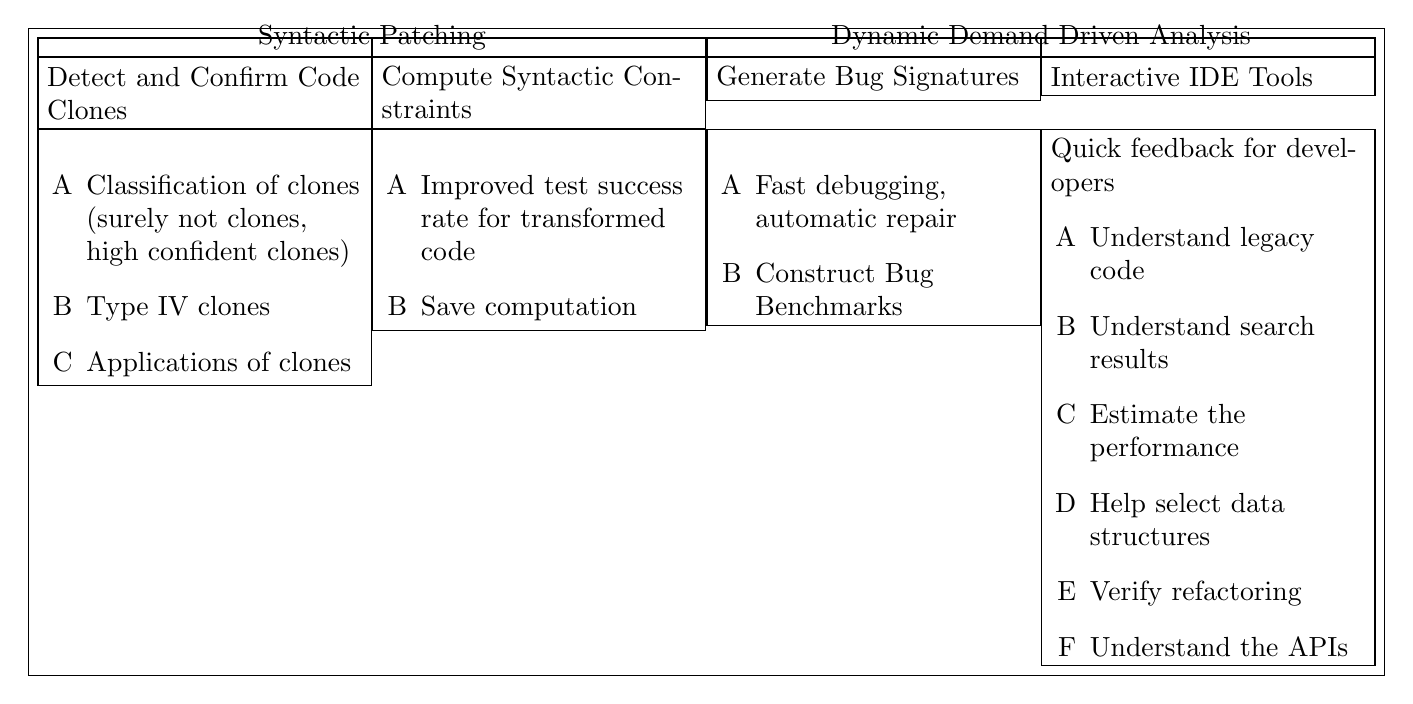
\begin{tikzpicture}
    % \matrix (tech) [
    %   draw,
    %   % inner ysep=0,
    %   every node/.style={text width=6cm,
    %     align=center,
    %     inner xsep=0.6667em,
    %     draw
    %   },
    %   ]{
    %   \node {Syntactic Patching};&
    %   \node {Dynamic Demand-Driven Analysis};\\
    % };
    \matrix (app) [
      draw,
      every node/.style={
        text width=4cm,
        draw
      },
      % below=0 of tech.south west,
      % matrix anchor=north west
      anchor=north west,
      ] {
      \node (n1) {};&
      \node (n2) {};&
      \node (n3) {};&
      \node (n4) {};\\
      \node {Detect and Confirm Code Clones};&
      \node {Compute Syntactic Constraints};&
      \node {Generate Bug Signatures};&
      \node {Interactive IDE Tools};\\
      \node {
        \begin{enumerate}[leftmargin=*,label=\Alph*]
        \item Classification of clones (surely not clones, high confident clones)
        \item Type IV clones
        \item Applications of clones
        \end{enumerate}
      };&
      \node {
        \begin{enumerate}[leftmargin=*,label=\Alph*]
        \item Improved test success rate for transformed code
        \item Save computation
        \end{enumerate}
      };&
      \node {
        \begin{enumerate}[leftmargin=*,label=\Alph*]
        \item Fast debugging, automatic repair
        \item Construct Bug Benchmarks
        \end{enumerate}
      };&
      \node {
        Quick feedback for developers
        \begin{enumerate}[leftmargin=*,label=\Alph*]
        \item Understand legacy code
        \item Understand search results
        \item Estimate the performance
        \item Help select data structures
        \item Verify refactoring
        \item Understand the APIs
        \end{enumerate}
      };\\
    };

    \node [fit=(n1) (n2)] {Syntactic Patching};
    \node [fit=(n3) (n4)] {Dynamic Demand-Driven Analysis};

  \end{tikzpicture}
\end{figure*}

\end{document}
